
\section{Intrusion Detection\label{sec:bg.ids}}

Organizations long relied on signature-based \glspl{ids} to detect intrusions.
These systems leverage a database of known attack patterns (\ie, \emph{signatures}) to identify malicious activities.
\Cref{lst:suricata} displays an example of a signature for detecting the Heartbleed vulnerability using Suricata, a popular open-source \gls{ids}.
This signature relies on dedicated code inside Suricata's engine that required extensive human intervention to develop.
It is consequently specific to Suricata.
Such limitations motivated the study of \gls{ml} for automatically extracting patterns from data, enabling the development of more flexible and adaptive \glspl{ids}.

\begin{listing}
  \begin{lstlisting}[gobble=4]
    alert tls any any -> any any (msg:"SURICATA TLS overflow heartbeat encountered, possible exploit attempt (heartbleed)"; flow:established; app-layer-event:tls.overflow_heartbeat_message; flowint:tls.anomaly.count,+,1; classtype:protocol-command-decode; reference:cve,2014-0160; sid:2230012; rev:1;)
  \end{lstlisting}
  \caption[
    Example of a Suricata signature for detecting the Heartbleed vulnerability.
  ]{
    Example of a Suricata signature for detecting the Heartbleed vulnerability\footnotemark{}.
    \label{lst:suricata} 
  }
\end{listing}

\footnotetext{\url{https://github.com/OISF/suricata/blob/master/rules/tls-events.rules}}

\Glspl{ids} can be broadly classified into two categories: \emph{misuse detection} and \emph{anomaly detection}.
Misuse detection refers to the identification of known attack patterns.
Signature-based \glspl{ids} fall into this category.
On the other hand, anomaly detection compares a normal profile (trained on nominal traffic) with observed events to determine if they are malicious~\cite{garcia-teodoro_Anomalybasednetworkintrusion_2009}.
This approach is \emph{de facto} more efficient for detecting novel attacks, but it is also more prone to false positives.

An analogy can be drawn between this classification and the two main paradigms of \gls{ml}: supervised and unsupervised learning.
In supervised learning, the model is trained on labeled data, where each sample is associated with a label.
Labels can be classes (binary or multi-class classification) or continuous values (regression).
Either way, the model's objective is to predict the label of unseen samples.
In unsupervised learning, no labels are provided.
The model's goal is to find patterns in the data, such as clusters or outliers.
In anomaly detection, the model is trained on normal data only, and its objective is to detect deviations from this normal profile.

Multiple \gls{ml} algorithms have been applied to intrusion detection, including \glspl{svm}, \glspl{rf}, and \glspl{ann}.
However, the rise of \gls{dl} has led to a significant improvement in the performance of \glspl{ids}.
\Gls{dl} is a subfield of \gls{ml} that focuses on learning representations of data through the use of neural networks.
In the following sections, we introduce the basics of \gls{dl} for intrusion detection, review the existing paradigms, and discuss the metrics and datasets used to evaluate these systems.


\subsection{Deep Learning for Intrusion Detection\label{sec:bg.ids.dl}}

\Gls{dl} present several advantages over traditional \gls{ml} algorithms.
Most notably, they automatically learn features from the data, reducing the need for manual feature engineering.
This is particularly useful in the context of intrusion detection, where the features are often complex, interdependent, and of unequal relevance.
The training data can range from network traffic to system logs depending on the type of mechanism used: network-based, host-based, or hybrid.
Yet, \glspl{nids} greatly outnumber other approaches in the literature, due the availability of network traffic datasets and the ease of deployment.

Most of the research on \gls{nids} use a representation known as \emph{unidirectional network flows} or \emph{netflows}, where a flow is defined as a sequence of packets sharing the same source and destination addresses, ports, and protocol.
Various features can be extracted from these flows, such as the number of packets, bytes, and the duration of the flow.
More details on the features used in \gls{nids} can be found in \Cref{sec:bg.ids.datasets}.
More generally, the dataset ($D$) is represented as a set of variables $X_i = \langle x_1, x_2, \ldots, x_n \rangle, i \in \llbracket 1, n \rrbracket $, where $x_j$ corresponds to the $j$-th feature.

\begin{figure}
  \centering
  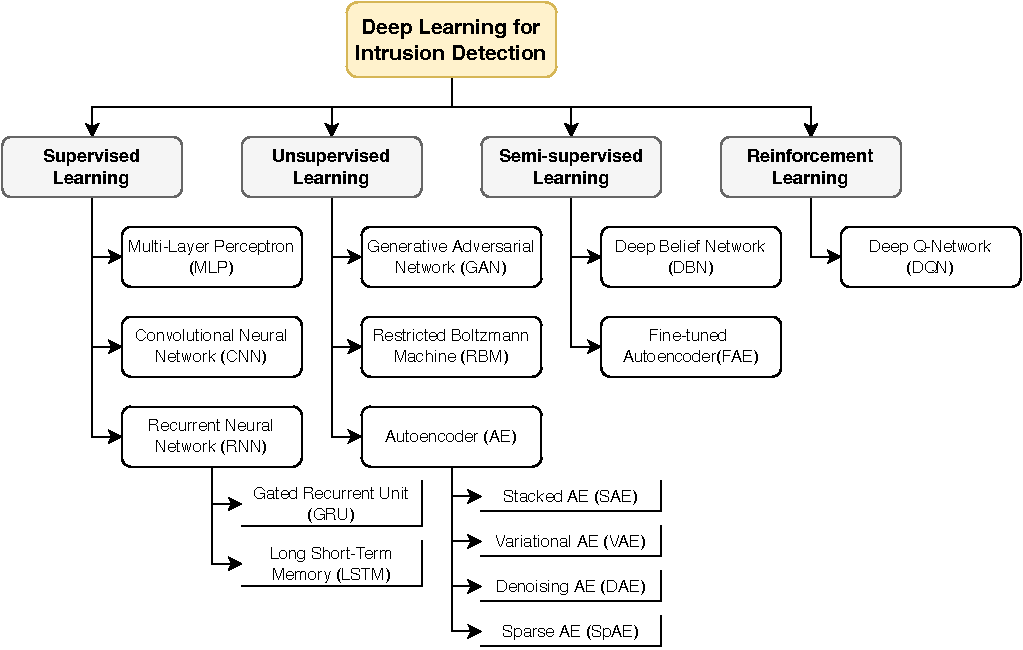
\includegraphics[width=0.8\textwidth]{figures/ml-taxonomy.pdf}
  \caption{
    Taxonomy of the main \gls{dl} paradigms.
    \label{fig:bg.taxonomy}
  }
\end{figure}

\subsubsection{Main \Gls{dl} Paradigms}

Because of their layered architecture, \glspl{dnn} can adopt different forms depending on the type of input data and the task at hand.
\Cref{fig:bg.taxonomy} presents the major families of \gls{dl} algorithms: supervised-, unsupervised-, and semi-supervised learning, and finally reinforcement learning.
While works exist on the application of reinforcement learning to intrusion detection~\needref{}, we focus on supervised and unsupervised learning in this thesis.
This section provides an overview of these paradigms, and define for each the learning problem in the context of intrusion detection.

\paragraph{Supervised Learning}

\begin{figure}
  \centering
  \includegraphics[width=.8\textwidth]{example-image-16x9}
  \caption{
    Workflow of training a \acrfull{mlp} for intrusion detection.
    \label{fig:bg.mlp}
  }
\end{figure}

Supervised learning is the most common approach in \gls{ml}, and refers to the training of a model on labeled data.
In the context of \glspl{ids}, practitioners usually seek to classify network flows into two classes (\emph{benign} and \emph{malicious}), which is a binary classification task.
Consequently, the dataset $D$ of size $n$ associates each sample $X_i$ with a label $y_i \in \lbrace 0,1 \rbrace $.
The model is trained to predict the label $\hat{y}$ of unseen samples.
To do so, we generally use a \gls{sgd}-based optimizer to minimize a loss function
\begin{equation} \label{eq:bg.loss}
  \mathcal{L}(w, X_i, y_i), i \in \llbracket 1, n \rrbracket.
\end{equation}
After computing the gradients $\nabla \mathcal{L}(w, X_i, y_i)$, they can update their model as
\begin{equation} \label{eq:bg.update}
  w^{t+1} \gets w^t - \eta \nabla \mathcal{L}(w, X_i, y_i),
\end{equation}
where $\eta$ is the learning rate, and $w$ the model's parameters, and $t$ the iteration.
The last layer usually uses \texttt{softmax} or \texttt{sigmoid} activation functions to output a probability of being in a class (normal or abnormal).
In the case of multi-class classification, the label is one-hot encoded\footnotemark{} into a vector $Y$ of size $c$ (the number of classes), and the \texttt{softmax} function is used.
Depending on the available features and the learning objective, various architectures can be used, such as \glspl{cnn} for high-dimensional data, or \glspl{rnn} for sequential data.
\Glspl{mlp} are the simplest and most common architecture used in \gls{ids}, and the one that we focus on in this thesis, although most concepts can be extended to other architectures.

\footnotetext{
  One-hot encoding is a binary representation of categorical variables, where each category is mapped to a binary vector.
  It is typically used in \gls{ml} to represent categorical data, such as the protocol type in netflows.
}

One of the main challenges in supervised learning is the availability of labeled data and its quality.
In the context of \gls{ids}, obtaining enough labeled data is particularly challenging, as labeling requires expert knowledge and is time-consuming.
Moreover, the class distribution is often unbalanced, with benign traffic being much more frequent than anomalies in the testing set~\cite{chandola_Anomalydetectionsurvey_2009}.
This issue is aggravated in siloed configurations, \ie, in which models can only be trained on locally-collected data.
This can lead to models that are skewed by the unbalanced class distribution~\cite{campos_EvaluatingFederatedLearning_2022}.

\begin{challenge}
  Locally collected data is often unbalanced, leading to models that are skewed by the class distribution.
  \label{chall:bias}
\end{challenge}


\paragraph{Unsupervised Learning}

\begin{figure}
  \centering
  \includegraphics[width=.8\textwidth]{example-image-16x9}
  \caption{
    Workflow of a \acrfull{sae} for intrusion detection.
    \label{fig:bg.mlp}
  }
\end{figure}

To circumvent the need for labeled data, unsupervised learning can be used.
Unsupervised \gls{ml} algorithms are typically used for clustering or outlier detection.
The \gls{dl} variants are rather used for feature extraction and dimensionality reduction, or anomaly detection.
To detect anomalies, \glspl{ae} can be trained on normal data only, and then used to see whether the reconstruction error of a new sample is above a certain threshold.
This builds on the assumption that
\begin{enumerate*}[(i)]
  \item benign traffic is much more frequent that anomalies in the testing set~\cite{chandola_Anomalydetectionsurvey_2009}; and
  \item abnormal packets are statistically different from normal ones.
\end{enumerate*}
In this scenario, the training dataset $D$ is composed of benign (\ie, normal) samples only and no associated label.
Given $X = \lbrace X_i | i \in \llbracket 1, n \rrbracket \rbrace $, the model is trained to minimize the reconstruction error $\mathcal{L}(X, \hat{X})$, where $\hat{X}$ is the output of the \gls{ae}.
A typical error function for this task is the \gls{mse}, expressed as:
\begin{equation}
  \text{MSE} = \frac{1}{n} \sum_{i=1}^{n} \left( X_i - \hat{X}_i \right)^2.
\end{equation}
Then the model can be updated using the same process described in \Cref{eq:bg.update}.
Different architectures of \glspl{ae} can be used, such as \glspl{sae} to improve the quality of the extracted features, or \glspl{dae} to improve the robustness of the model. 
To detect anomalies, the reconstruction error of a new sample is compared to a threshold $\tau$ defined during the training phase on validation data.
A high reconstruction error indicates that the considered samples is too \emph{far} from the training data, and can indicate an anomaly.
The performance of the model and its threshold can then be evaluated using a labelled test set.

While unsupervised learning is particularly useful for detecting novel attacks, it is also more prone to misclassification.
Local data in the real-world is likely to be collected on devices with little variance, \eg same brand, same protocols, or use cases.
This can lead to a normal profile that is too specific to the local environment, and thus would raise alerts as soon as a change occurs~\cite{liu_MachineLearningDeep_2019}.

\begin{challenge}
  Local data is specific to the environment, increasing the risk of false positives when changes occur.
  \label{chall:specificity}
\end{challenge}


\paragraph{Semi-supervised Learning}

Semi-supervised learning is a hybrid approach where only a small part of the training data is labeled.
This approach is particularly useful in the context of \gls{ids}, where labeled data is scarce.
A common strategy is to train an \gls{ae} on the full dataset to learn the optimal representation of the data, and use the encoder part with a classifier to predict the label of the samples~\cite{aouedi_SemisupervisedStackedAutoencoder_2020}.
Other known model architectures for semi-supervised learning include \glspl{dbn}, where multiple layers of \glspl{rbm} are stacked to form a deep network that extracts features from the data.
The model is then fine-tuned using the labeled data for classification purposes.


\subsection{Datasets\label{sec:bg.ids.datasets}}

Datasets are essential in intrusion detection, as they allow researchers to evaluate and compare their solutions.
This is even more critical when leveraging \gls{ml} and \gls{dl} techniques, as the performance of these models is highly dependent on the quality and quantity of the training data.
Until the mid-2010s, the most common dataset used for intrusion detection was the {KDD'99} dataset~\cite{kddcup99}, built for the KDD Cup 1999 competition using the DARPA 1998 dataset.
\Textcite{tavallaee_detailedanalysisKDD_2009} published an updated version of the dataset, called NSL-KDD, which removes duplicates and corrects some errors in the original dataset.
However, NSL-KDD is still based on the original DARPA 1998 dataset, and is considered outdated by today's standards.

Since 2015 with the publication of the UNSW-NB15 dataset~\cite{moustafa_UNSWNB15comprehensivedata_2015}, new datasets have been developed to address the limitations of the KDD'99 and NSL-KDD datasets, such as the lack of realism\footnotemark of the generated traffic, the lack of attack diversity, and the scale of the experiments.
\Cref{tbl:datasets} presents the most common feature-based datasets for \glspl{nids}, along with their characteristics.
Two teams have been particularly active in this area: the Intelligent Security Group (ISG)~\cite{moustafa_UNSWNB15comprehensivedata_2015,koroniotis_developmentrealisticbotnet_2019,moustafa_newdistributedarchitecture_2021} at the University of New South Wales, Australia, and the Canadian Institute for Cybersecurity (CIC)~\cite{sharafaldin_GeneratingNewIntrusion_2018} at the University of New Brunswick, Canada.
They brought the most used datasets in the field in recent years, UNWS-NB15 and CICIDS2017, respectively.

\footnotetext{
  In regard to modern networks.
  Indeed, the DARPA 1998 dataset simulates multiple workstations in a military environment, using the US Air Force Research Laboratory's testbed.
  The technologies deployed where representative of the state of the art at the time.
}

\begin{table}
  \centering
  \caption{
    Most common feature-based datasets for \glspl{nids}.
    \label{tbl:datasets}  
  }
  \hfill
\begin{minipage}{.48\textwidth}
  \small
  \begin{tabularx}{\linewidth}{lXrr}
    \toprule % ------------------------------------
    \multicolumn{1}{c}{\textbf{Class}} & & \multicolumn{1}{c}{\textbf{Sampled}} & \multicolumn{1}{c}{\textbf{Full}} \\
    \midrule % ---------------------------------
    Benign         & & 880,623   & 16,635,567 \\
    DDoS           & & 73,558    & 1,390,270  \\
    DoS            & & 25,574    & 483,999    \\
    Bot            & & 7,595     & 143,097    \\
    Brute Force    & & 6,525     & 123,982    \\
    Infiltration   & & 6,108     & 116,361    \\
    Injection      & & 17        & 432        \\
    & & & \\
    & & & \\
    & & & \\
    \midrule % ---------------------------------
    \textbf{Total} & & 1,000,000 & 18,893,708 \\
    \bottomrule % ---------------------------------
  \end{tabularx}
\end{minipage}
\hfill
\begin{minipage}{.48\textwidth}
  \small
  \begin{tabularx}{\linewidth}{lXrr}
    \toprule % ---------------------------------
    \multicolumn{1}{c}{\textbf{Class}} & & \multicolumn{1}{c}{\textbf{Sampled}} & \multicolumn{1}{c}{\textbf{Full}} \\
    \midrule % ---------------------------------
    Benign           & & 960,078  & 2,295,222   \\
    Exploits         & & 13,187   & 31,551      \\
    Fuzzers          & & 9,377    & 22,310      \\
    Generic          & & 6,976    & 16,560      \\
    Reconnaissance   & & 5,352    & 12,779      \\
    DoS              & & 2,455    & 5,794       \\
    Analysis         & & 969      & 2,299       \\
    Backdoor         & & 925      & 2,169       \\
    Shellcode        & & 617      & 1,427       \\
    Worms            & & 64       & 164         \\
    \midrule % ---------------------------------
    \textbf{Total}   & & 1,000,000 & 2,390,275  \\
    \bottomrule % ------------------------------
  \end{tabularx}
\end{minipage}
\hfill
  \end{table}

\paragraph{Provided features}

Because most of the datasets presented in \Cref{tbl:datasets} are made to train and evaluate \glspl{ml} models, they rely on a set of features extracted from the network traffic.
Some also include the original network captures (PCAPs) for further analysis, or complementary system logs for correlation purposes.
Two non-exclusive approaches can be used to produce these features: feature extraction and feature selection.

\begin{description}
  \item[Feature extraction] refers to the computation of numerical characteristics after the data collection; \eg, \gls{iat} or number of packets per device in the context of traffic monitoring.
  Most modern dataset use existing \glspl{ids} to extract these features, such as Zeek\footnote{Formerly known as Bro, available at: \url{https://www.zeek.org/}} or Argus\footnote{Available at: \url{https://openargus.org/argus-ids}}.
  The resulting data are network flows, aggregating the information of multiple packets into a single record.

  \item[Feature selection] relates to the selection of the relevant features for a given task.
  This is particularly useful in the context of \gls{ml}, where irrelevant or redundant features can degrade the performance of the model.
  For instance, Edge-IIoTset~\cite{ferrag_EdgeIIoTsetNewComprehensive_2022} contains 61 features, selected from a pool of 1176 based on feature correlation.
\end{description}

The choice of features is critical for the performance of the model, although \gls{dl} models make this process less relevant due to their ability to filter out irrelevant features.
Yet, because each dataset comes with its own set of features, it is difficult to compare the performance of models across datasets.
Recently, \textcite{sarhan_StandardFeatureSet_2022} proposed a standardized feature set for intrusion detection based on NetFlow V9~\cite{rfc3954} format.
They used nProbe\footnote{Available at: \url{https://www.ntop.org/products/traffic-analysis/nprobe/}} to convert four known \gls{ids} datasets to this format: \ie, UNSW-NB15~\cite{moustafa_UNSWNB15comprehensivedata_2015}, Bot-IoT~\cite{koroniotis_developmentrealisticbotnet_2019}, ToN\_IoT~\cite{moustafa_newdistributedarchitecture_2021}, and CSE-CIC-IDS2018~\cite{sharafaldin_GeneratingNewIntrusion_2018}.
The NF-V2 datasets contain 43 features extracted from flow characteristics, such as duration or packet length, and some others that are protocols-specific.
The uniform feature set across datasets allows the evaluation of \gls{ml} models across independently generated datasets.

\paragraph{Use cases}

Until 2017 included, most datasets aim at simulating a \emph{typical} network environment, such as deployed in an organization.
This is the case for KDD'99, NSL-KDD, UNSW-NB15, and CIDDS 1 and 2, and CICIDS2017.
Since, the focus progressively shifts towards more specific use cases, notably with the generalization of \gls{iot} devices.
These datasets include protocols that are not present in traditional IT-oriented networks, such as MQTT or CoAP.
This is the case for Bot-IoT~\cite{koroniotis_developmentrealisticbotnet_2019}, ToN\_IoT~\cite{moustafa_newdistributedarchitecture_2021}, and Edge-IIoTset~\cite{ferrag_EdgeIIoTsetNewComprehensive_2022}.



% \footnote{\url{https://www.rfc-editor.org/rfc/rfc3954}} Netflow V9

\subsection{Metrics\label{sec:bg.ids.metrics}}

Most research on \gls{ml} for intrusion detection relies on the same set of metrics to assess, validate, and compare their solutions~\cite{chaabouni_NetworkIntrusionDetection_2019,faraj_Taxonomychallengesmachine_2020,buczak_SurveyDataMining_2016}.
Most of these metrics are derived from the confusion matrix (see \Cref{tbl:bg.conf}), which is a table that summarizes the performance of a classification model along the different classes.
To compute the confusion matrix, the model's predictions ($\hat{y}$) are compared to the true labels ($y$, the ground truth) of the samples.
All the metrics presented in this section are defined for binary classification, but can be extended to multi-class classification~\cite{buczak_SurveyDataMining_2016}.

\begin{table}
  \centering
  \begin{tabular}{cc|c|c|}
    \multicolumn{2}{c}{} & \multicolumn{2}{c}{\textbf{Predicted}} \\
    \multirow{3}{*}{\rotatebox{90}{\textbf{Actual}}} & & \textbf{Positive} & \textbf{Negative} \\
    \cline{2-4}
     & \textbf{Positive} & \glspl{tp} & \glspl{fn} \\
    \cline{2-4}
    & \textbf{Negative} & \glspl{fp} & \glspl{tn} \\
    \cline{2-4}
  \end{tabular}
  \caption{
    Confusion matrix for binary classification.
    \label{tbl:bg.conf}
  }
\end{table}

\begin{enumerate}[(1)]
  \item \emph{Accuracy} represents the proportion of correctly classified items.
  It is the ability for the system to correctly distinguish abnormal traffic from legitimate one.
  \begin{equation*}
    Accuracy = \frac{TP+TN}{P+N}
  \end{equation*}

  \item \emph{Precision}, or \gls{ppv}, is the proportion of correct positive cases among all the cases that have been categorized as positive.
  \begin{equation*}
    Precision = \frac{TP}{TP+FP}
  \end{equation*}

  \item \emph{Recall}, or \gls{tpr} represents the proportion of true positive cases that have been correctly categorized.
  \begin{equation*}
    Recall = \frac{TP}{P} = \frac{TP}{TP+FN}
  \end{equation*}

  \item \emph{Specificity}, or \gls{tnr}, is the proportion of negative cases that has been correctly categorized.
  \begin{equation*}
    Specificity = \frac{TN}{P} = \frac{TN}{TN+FP}
  \end{equation*}

  \item \emph{Fallout}, or \gls{fpr}, represents the proportion of the positive cases that should have been categorized as negative.
  A high \gls{fpr} often requires human intervention after the classification task to filter out the false positive.

  \begin{equation*}
    Fallout = \frac{FP}{N} = \frac{FP}{FP+TN}
  \end{equation*}

  \item \emph{Miss rate}, or \gls{fnr}, relates to the proportion of positive cases that have not been categorized as such.
  In the context of \glspl{ids}, it represents an attack that has been missed by the system.
  Thus, it is a critical metric for this use case.
  \begin{equation*}
    Miss\ rate = \frac{FN}{P} = \frac{FN}{FN+TP}
  \end{equation*}

  \item \emph{F1-Score} is the harmonic mean of precision and recall.
  It is often used to measure ML algorithm, but is also criticized because of the equal importance it gives to both precision and recall~\cite{hand_noteusingFmeasure_2018}.
  \begin{equation*}
    F_1 = 2 \times \frac{Precision \times Recall}{Precision+Recall}
  \end{equation*}

  \item \emph{\gls{mcc}} is an adaptation of the \emph{Phi} (\(\phi\)) coefficient to confusion matrices.
  While being mathematically identical, the term is often preferred by the \gls{ml} community.
  The \gls{mcc} has significant advantages over the other metrics, as it covers all four categories of the confusion matrix~\cite{chicco_advantagesMatthewscorrelation_2020}.
  Thus, a high score can only be obtained with high \(TP\) and \(TN\), and low \(FP\) and \(FN\).

  \begin{equation*}
      MCC = \dfrac{TP \times TN - FP \times FN}{\sqrt{(TP + FP)(TP + FN)(TN + FP)(TN + FN)}}
  \end{equation*}%

\end{enumerate}